%%This is a very basic article template.
%%There is just one section and two subsections.
\documentclass[11pt,a4paper]{report}  	%% hvad for en type dokument er det?

%%preamble
\usepackage[utf8]{inputenc}
\usepackage{fancyhdr}
\usepackage[titletoc]{appendix}
\usepackage{lastpage}
\usepackage{hyperref}
\pagestyle{fancy}
\bibliographystyle{plain}	%%style på refferencer
\renewcommand{\chaptername}{}
\renewcommand{\thechapter}{}
\setcounter{tocdepth}{1}

%%end preamble
%%--------------------------------------------------------------------------------
\begin{document}			%%begynd dokumentet
%%--------------------------------------------------------------------------------
\nocite{*}					%%erstatter citeringer i texten med reference tal	

\pagenumbering{Alph}		%%fixes hyperref pagenumbering error (sets it to uppercase
							%% letters)
\thispagestyle{empty}
\begin{titlepage}
\bfseries
\begin{flushleft}
Projectopgave efterår 2013 - jan 2014\\
02312-14 Indledende programmering\\
02313 Udviklingsmetoder til IT-Systemer.\\
Projektnavn: CDIO delopgave 3\\
Gruppe nr: 51.\\
Afleveringsfrist: mandag den 02/12 2013 Kl. 5:00\\
Denne rapport er afleveret via Campusnet (der skrives ikke under)\\
Denne rapport indeholder \pageref{LastPage} sider exkl. denne side.\\
\end{flushleft}
\vspace{5\baselineskip}
\begin{center}
\begin{tabular}{l}
s123064, Nielsen, Martin\\
\\
s130045, Kheder, Mustafa\\
\\
s103185, Sløgedal, Magnus B.\\
\\
s134000, Budtz, Christian\\
\\
s133984, Freudendahl, Jens-Ulrik\\
\\
s134004, Vørmadal, Rúni Egholm\\
\end{tabular}
\end{center}

\end{titlepage}

\newpage %%contains \thispagestyle{empty} so no numbers

\pagenumbering{arabic}		%%fixes hyperref pagenumbering error (sets it back to
							%% numbers)
\tableofcontents

\chapter{Inledning}
I IOOuterActive har vi fået en ny ordre fra kunden, som involvere at udvide det
sidste spil vi lavede (CDIO.del2)til et rigtigt brætspil, med nye felt typer,
samt at brug af polymorfi og muligheden for at købe felter.\\
\indent Denne rapport er skrevet til personer med en generel viden omkring UML
(Unified Modeling Language) og programmeringssproget Java. Målet med denne
rapport er at dokumentere vores arbejde på denne ordre i IOOuterActive.\\
\indent Til udarbejdning af rapporten og programmet har vi brugt følgende
værktøjer:
\begin{itemize}
  \item Eclipse - Vores valgte development environment.
  \item GitHub - Vores version control system of choice.
  \item Google Docs - for at synkronisere rapportskrivningen.
  \item LaTeX - For at få et pænere final product.
  \item Software Ideas Modeller - For vores UML-diagrammer.
\end{itemize}
Rapporten beskriver følgende emner:
\begin{itemize}
  \item Krav - Vi har foretaget en kravspecificering og en use-case analyse,
  hvor vi kommer ind på en fully dressed use-case beskrivelse  af  “Land on fleet”,
  for at give os en bedre forståelse af kundens ønsker, og omfanget af
  opgaven.
  \item Design - Vi har dokumenteret vores design i UML form for at give os et
  overblik over programmet og fastlægge placeringen af koden. vi bestræber os på
  at overholde GRASP koncepterne i designet.
  \item Implementering - Vi har implementeret det valgte design. Dette er blevet
  dokumenteret i rapporten ved hjælp af beskrivelser af alle klasserne, en
  forklaring af konceptet arv i en objekt orienteret sammenhæng samt termet
  abstract.
  \item Test - Vi har testet programmet, både manuelt og via JUnit, og benyttet
  FURPS+ for at prøve at sikre en god maintenance og operation af programmet.
\end{itemize}

\chapter{Analyse}
Kundens vision er at få leveret et terningspil, der kan spilles af 2-6 spillere.
Spillerne rykker rundt på et ringformet spillebræt med 21 felter. Hver spiller
starter med 30.000. Spillet slutter når kun en spiller ikke er bankerot.\\
\FloatBarrier
\begin{figure}[h]
\section*{Domænemodel}
\addcontentsline{toc}{subsection}{Domænemodel}
\centering
\makebox[\textwidth]{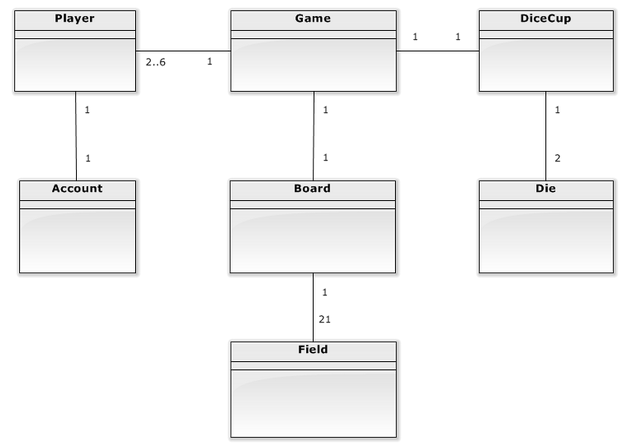
\includegraphics[width=\textwidth]{DOM_51_del3}}
\caption{\emph{Domæne model}: Viser hvordan spillet hænger sammen ude i den
virkelige verden. Det man ikke kan se her, er at Field, indeholder forskellige slags
felter.}
\end{figure}
\FloatBarrier
\section*{Use Cases}
\addcontentsline{toc}{subsection}{Use Cases}
Vi har valgt at betragte spillet som bestående af en overordnet spil ‘use case’,
hvor spillerne efter tur slår med terninger og rykker rundt på felterne. Vi
betragter hvert ophold på et felt som en separat sub use case, der igen udvides
i flere trin (se Use case diagram). Nogle af felterne kan ejes og modelleres
derfor i en separat use case - der igen er delt op i flere typer af felter - alt
efter hvordan lejen af feltet afgøres.\\
\indent Af kunden er det specificeret at netop ‘Land on Fleet’ skal være særligt
grundigt dokumenteret - ‘fully dressed’. Vi har valgt at beskrive en sub use
case, ‘Land on Field’, der er højere i hierarkiet, som ‘fully dressed’, idet der
er mange generelle elementer, der går igen i de forskellige use cases. ‘Land on
Fleet’ er således beskrevet som en extension af den mere generelle ‘Land on
Ownable Field’, der igen er et specialtilfælde af ‘Land on Field’.\\
\FloatBarrier
\begin{figure}[h]
\section*{Use Case Diagram}
\addcontentsline{toc}{subsection}{Use Case Diagram}
\centering
\makebox[\textwidth]{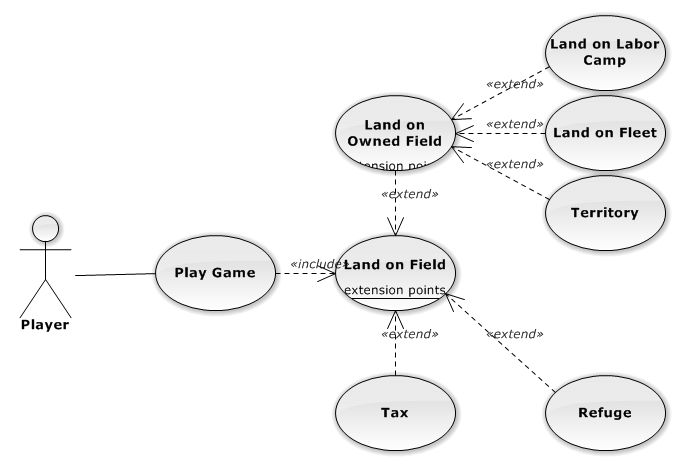
\includegraphics[width=\textwidth]{Usecasediagram1}}
\caption{\emph{Use Case Diagram}: Vi har valgt at beskrive ‘Land on Field’ som
en include i Play Game - selvom der ikke er flere use cases der include’r ‘Land on
Field’. Dette er gjort for at synliggøre relationen mellem sub use cases.}
\end{figure}
\FloatBarrier
\section*{Main Use Case ‘Spil Terningspil’}
\addcontentsline{toc}{subsection}{Main Use Case ‘Spil Terningspil’}
\begin{enumerate}
  \item Spillerne starter spillet og vælger hvor mange spillere de vil være.
  \item De indtaster spillernavne.
  \item Spillerne starter med 30000 points hver. Spillebrættet har 21 felter,
  der ligger i en ring. Nogle af felterne kan ejes af spillerne.
  \item Spillerne slår efter tur med 2 terninger og rykker summens øjne frem på
  spillebrættet. Alt efter hvilket felt man lander på mister eller får man penge
  og en ejer modtager evt. pengene. Se sub use case ‘Land on Field’
  \item Spillet slutter når alle undtagen én spiller er fallit og den
  tilbageværende spiller vinder.
\end{enumerate}
\textbf{Extension:}\\
1a. Spillerne kan vælge sprog\footnote{Er ikke specificeret i oplægget, men vi
har valgt at implementere det, som en ekstra udfordring.}.\\
\\
\textbf{\large Sub Use Case ‘Land on Field’ (fully dressed)}\\
Included in Main Use Case (4.)\\
\textbf{Scope:} Terningspil.\\
\textbf{Level:} Subfunction.\\
\textbf{Primary Actor:} Aktive spiller (spilleren der har tur).\\
\textbf{Stakeholders and Interests:} Alle spillere:
\begin{itemize}
  \item Er interesserede i at spillerne får opdateret deres pengebeholdning i
  overensstemmelse med reglerne for felttypen.
  \item Er interesserede i at finde ud af om den aktive spiller går fallit.
  \item Forventer entydig kommunikation af resultatet af at lande på feltet.
\end{itemize}
\textbf{Preconditions:} Spillet er startet og der er en aktiv spiller (der har
turen), der lander på et felt.\\
\textbf{Postconditions:} De involverede spillers pengebeholdning bliver
opdateret. Spillerens tur afsluttes.\\
\textbf{Main Success Scenario:}
\begin{enumerate}
  \item Spilleren lander på feltet.
  \item Spillerens penge beholdning opdateres.
  \item Spillerens tur afsluttes.
\end{enumerate} 
\textbf{Extensions:}\\
2a. Feltet kan ejes - Sub Use Case Land on Ownable Field.\\
2b. Feltet er af typen ‘Tax’ - Sub Use Case Land on Tax.\\
2c. Feltet er af typen ‘Refuge’ - Sub Use Case Land on Refuge\\
2d. Spilleren går fallit
\begin{enumerate}
  \item Spillerens penge sættes til 0.
  \item Spilleren får ikke flere ture.
\end{enumerate}
\textbf{Special Requirements, Technology and Data variations list.}\\
Der er i den givne opgave ikke stillet krav inden for ovenstående.\\
\textbf{Frequency of occurrence.}\\
Hver runde i spillet.\\
\textbf{Open Issues.}\\
Beskrevet under afklaring og antagelser.\\
\\
\textbf{\large Sub Use Case Land on Ownable Field}\\
Extends \emph{Land on Field.}\\
Feltet kan ejes.
\begin{enumerate}
  \item Feltet har ingen ejer.
  \begin{enumerate}
    \item Spilleren tilbydes at købe feltet, har tilstrækkeligt med penge og
    køber feltet.
    \begin{enumerate}
      \item Spilleren bliver ejer af feltet.
      \item Prisen for feltet fratrækkes spillerens saldo.
    \end{enumerate}
    \item Spilleren tilbydes at købe feltet, har tilstrækkeligt med penge, men
    køber ikke feltet.
    \item Spilleren har ikke tilstrækkeligt med penge til at købe feltet.
  \end{enumerate}  
  \item Feltet er allerede ejet af spilleren.
  \item Feltet er ejet af en anden spiller.
  \begin{enumerate}
    \item Spilleren betaler leje til ejeren.
  \end{enumerate}
\end{enumerate}
\textbf{Extensions:}\\
3.1a. Feltet er et ‘Territory’ - Sub Use Case Land on Territory.\\
3.1b. Feltet er et ‘Labor Camp’ - Sub Use Case Land on Labor Camp.\\
3.1c. Feltet er et ‘Fleet’ - Sub Use Case Land on Fleet.\\
3.1d. Spilleren har ikke tilstrækkeligt med penge til at betale ejeren.
\begin{enumerate}
  \item Ejeren får spillerens resterende penge.
  \item Spilleren går fallit.
\end{enumerate}
\\
\textbf{\large Sub Use Case Land on Territory}\\
Extends \emph{Land on Ownable Field.}\\
1. Spilleren der lander på ‘Territory’ betaler ejeren et foruddefineret
beløb.\\
\\
\textbf{\large Sub Use Case Land on Labor Camp}\\
Extends \emph{Land on Ownable Field.}\\
1. Spilleren der lander på ‘Labor Camp’ betaler ejeren 100 gange øjnene på det
slag, der har bragt ham til feltet.\\
\\
\textbf{\large Sub Use Case Land on Fleet}\\
Extends \emph{Land on Ownable Field.}\\
1. Spilleren der lander på ‘Fleet’ betaler ejeren $2^n \cdot 250 $, hvor n er
antallet af fleets, som ejeren ejer.\\
\\
\textbf{\large Sub Use Case Land on Tax}\\
Extends \emph{Land on Field.}\\
1. Spilleren mister et foruddefineret beløb.\\
\textbf{Extension:}
1a. På nogle ‘Tax’ felter kan spilleren i stedet vælge at betale en procentdel
af sin samlede formue\\
\\
\textbf{\large Sub Use Case Land on Refuge}\\
Extends \emph{Land on Field.}\\
Spilleren modtager et foruddefineret beløb.\\
\section*{Non funktionelle krav}
\addcontentsline{toc}{subsection}{Non funktionelle krav}
I den givne opgave er der det er et krav at der er udarbejdet
Kravspecificering:
\begin{enumerate}
  \item Et use-case diagram og use-case beskrivelser. Som minimum skal ”Land on
  fleet” være fully dressed.
  \item Domæne-model og BCE-diagram
\end{enumerate}
Kodemæssigt forlanges:
\begin{enumerate}
  \item Lav passende konstruktører.
  \item Lav passende get og set metoder.
  \item Lav passende toString metoder.
  \item Lav en klasse GameBoard der kan indeholde alle felterne i et array.
  \item Tilføj en toString metode der udskriver alle felterne i arrayet.
  \item Lav en Junit test til hver af felttypernes ”landOnField”-metode.
  \item Lav det spil kunden har bedt om med de klasser I nu har.
  \item Benyt den udleverede GUI.
\end{enumerate}
Designmæssigt forlanges:
\begin{enumerate}
  \item DSD’er (Design Sekvens Diagrammer). Som minimum ”Land on fleet”.
  \item Forklaring af arv, keywordet abstract, og konceptet i at implementere
  landOnField metoder i både super og subclasses (override).
  \item Dokumentation for test med screenshots.
  \item Dokumentation for overholdt GRASP.
\end{enumerate}
\section*{Afklaring og antagelser}
\addcontentsline{toc}{subsection}{Afklaring og antagelser}
\begin{enumerate}
  \item Vi adspurgte kunden om felterne skulle ligge i nummereret rækkefølge på
  brættet. Kunden svarede at det var valgfrit, men så gerne at de lå tilfældigt.
  \item Vi antager at alle spillere starter på første felt
  \item Vi antager at alle felter bevarer deres værdi når de er købt - således
  at det koster 10\% af ens saldo + 10\% af indkøbsprisen for de Tax felter hvor
  det er muligt at betale 10\% af sin formue.
\end{enumerate}
\section*{Ikke honorerede krav}
\addcontentsline{toc}{subsection}{Ikke honorerede krav}
Vi har forsøgt at honorere alle krav.\\

\chapter{Design}
Ud fra ovenstående use case analyser er vi fortsat med at designe en løsning på
opgaven. I lighed med den foregående opgave har vi besluttet os for en løsning
med en decorator, der sørger for at gøre det let at oversætte spillet til et
andet sprog. I vores tilfælde har vi en lidt speciel GUI, der - imodsætning til
en ‘normal’ GUI - afventer en forespørgsel fra vores Gamecontroller/Decorator.
Dette afspejles i vores BCE diagram. I vores BCE diagram er lagt op til en
central controller, hvilket vi dog har valgt at ‘bøje’ lidt i
klassediagrammet.\\
\FloatBarrier
\begin{figure}[h]
\section*{BCE Diagram}
\addcontentsline{toc}{subsection}{BCE Diagram}
\centering
\noindent 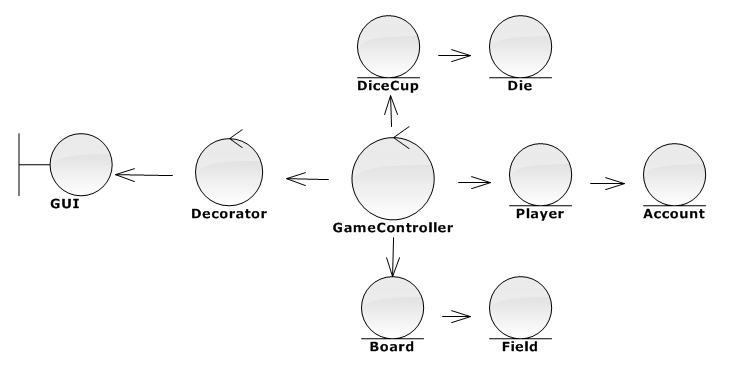
\includegraphics[width=\linewidth]{Robustnessdiagram1}
\caption{\emph{BCE diagram}: Bemærk den lidt usædvanlige
relation mellem GameController Decorator og GUI. GUI afventer en forespørgsel
fra Gamecontroller/Decorator, hvorfor pilen vender modsat vanlig interaktion med
en GUI.}
\end{figure}
\FloatBarrier
\begin{figure}[h]
\section*{Design Klasse diagram}
\addcontentsline{toc}{subsection}{Design Klasse Diagram}
\centering
\noindent 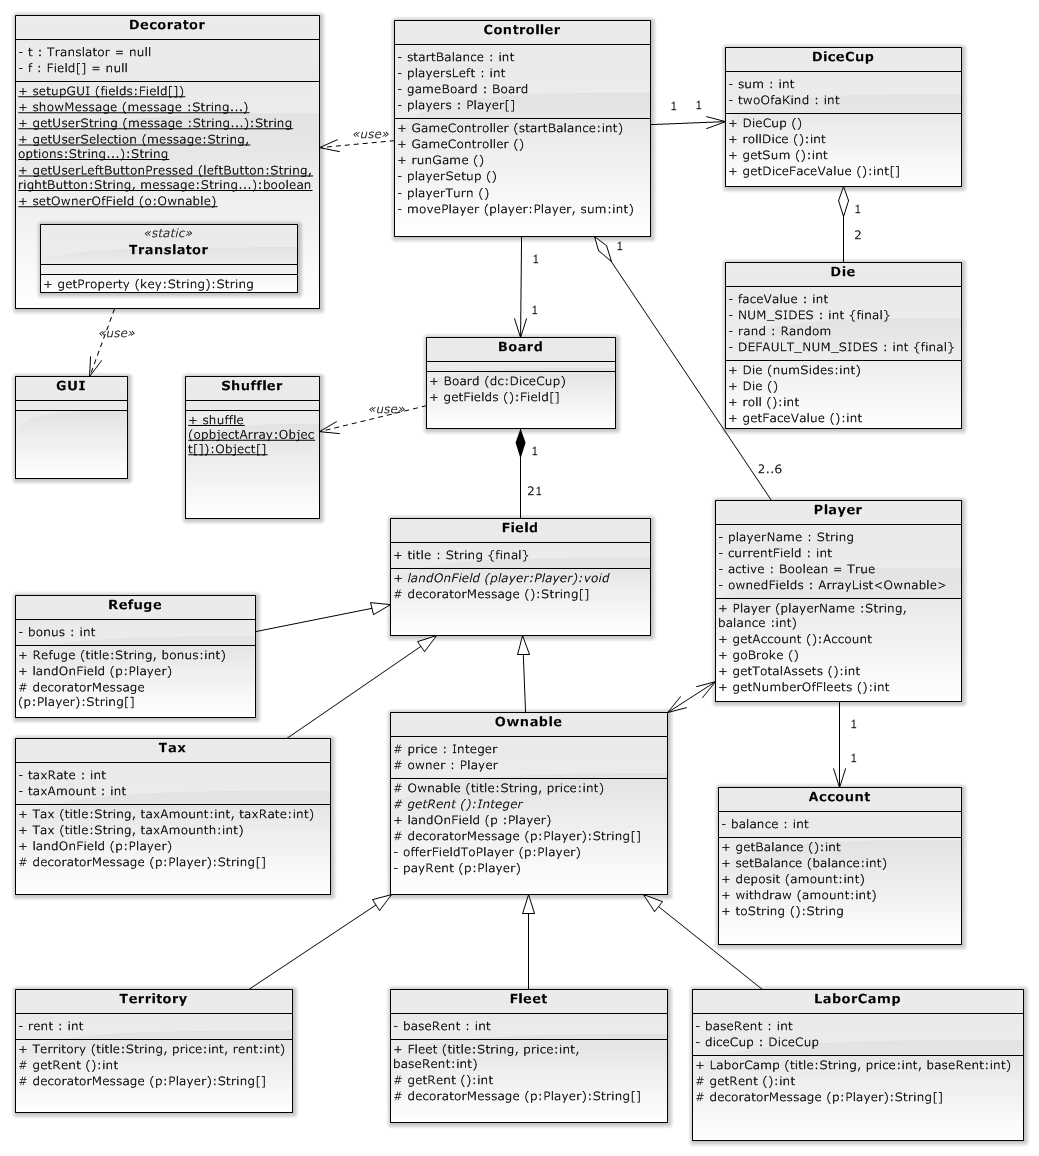
\includegraphics[width=\linewidth]{Classdiagram1}
\caption{\emph{Design klasse diagram}: Flere ‘use’ relationer er udeladt for
overskuelighedens skyld. Således er der en ‘use’ relation fra Refuge, Tax,
Territory, Fleet, LaborCamp og Player til Decorator, der er en statisk klasse og
dermed kan tilgås globalt. Desuden er udeladt en association fra LaborCamp til
DiceCup, der bruges til at tilgå terningslaget.\\
I design klassediagrammet har vi udviklet BCE modellen yderligere, så
den rent faktisk afspejler koden. Der er dukket to nye hjælperklasser op - Shuffler og
Translator, der er henholdsvis en statisk hjælperklasse, der kan blande objekter
i et array og en indre klasse, der oversætter Strings via en properties fil,
der er sprogspecifik.}
\end{figure}
\FloatBarrier
\section*{Arv, Polymorfi og Abstract}
\addcontentsline{toc}{subsection}{Arv, Polymorfi og Abstract}
Klassen Field er nu videreudviklet til at have et arvehieraki, der reflekterer
at Fields er forskellige, men har ensartede attributter og metoder - altså
udviser polymorfi. Polymorfi er: \emph{“Muligheden for at bruge den samme kode på
flere forskellige objekter, og for at den kode kan opføre sig forskelligt alt
efter hvilket objekt der er tale om.”}\cite{buildingJava} I vores kode bruger vi
polymorfi til at differentiere mellem forskellige felters landOnField metode, og
vi bruger det i decoratorMessage til at bestemme hvilket text output, der skal
sendes til vores Decorator og videre til GUI.\\
\indent Alle felterne har attributten ‘title’ tilfælles, hvorfor den ligger i
øverste klasse ‘Field’ i arvehierarkiet. Desuden implementerer Field metoden
decoratorMessage(), og en abstrakt metode - landOnField(). Det at en metode er
abstrakt, betyder at den ikke bliver  implementeret i den klasse hvor den er
erklæret abstrakt - det vil sige den ikke  har en metode-body. Fordelen ved at
erklære en abstrakt metode i superklassen er  at man tvinger sub klasser til at
implementere klassen, og man derfor kan være  sikker på at alle subklasser har
metoden. Når en metode bliver erklæret abstrakt  skal klassen også erklæres
abstract. For en klasse betyder dette at den ikke  længere kan instantieres, så
hvis man skal bruge den bliver man nødt til at  nedarve den til en sub-klasse.\\
\indent Ownable er super klasse for de felter  der kan købes - og en sub klasse
af Field. Det er meningsfyldt, da de alle skal  kunne købes - altså har en pris,
‘price’ og en ejer ‘owner’ og skal implementere  metoder til at beregne leje -
getRent().\\
\indent Med de to super klasser Field og  Ownable har vi opnået at kunne
genbruge så meget kode som muligt og undgår  dermed at skulle rette flere steder
i koden når metoderne skal opdateres.\\
\FloatBarrier
\section*{Sekvensdiagrammer}
\addcontentsline{toc}{subsection}{Sekvensdiagrammer}
Ud fra uses cases og klasse diagram har vi forsøgt at analysere flowet i spillet
og modelleret det i de følgende sekvensdiagrammer.
\begin{figure}[h]
\centering
\noindent 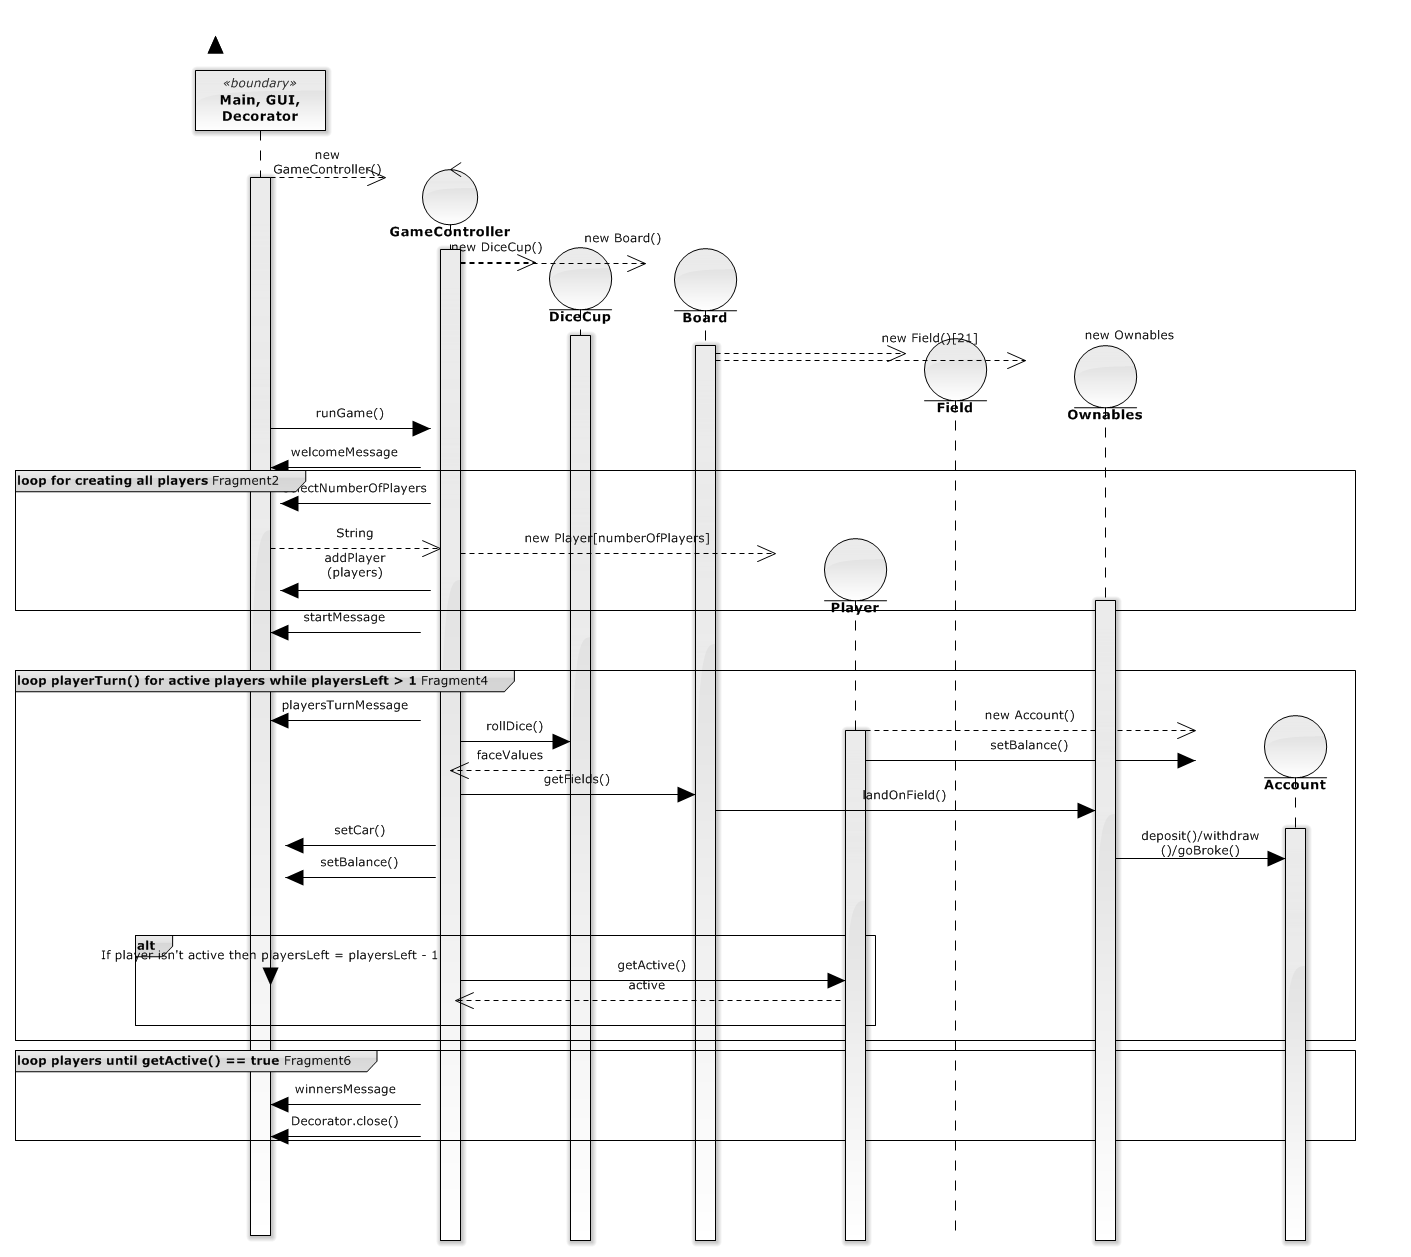
\includegraphics[width=\linewidth]{DesignSequenceDiagram}
\caption{\emph{Sekvensdiagram 1}: Play Game.}
\end{figure}
\FloatBarrier
\begin{figure}[h]
\centering
\noindent 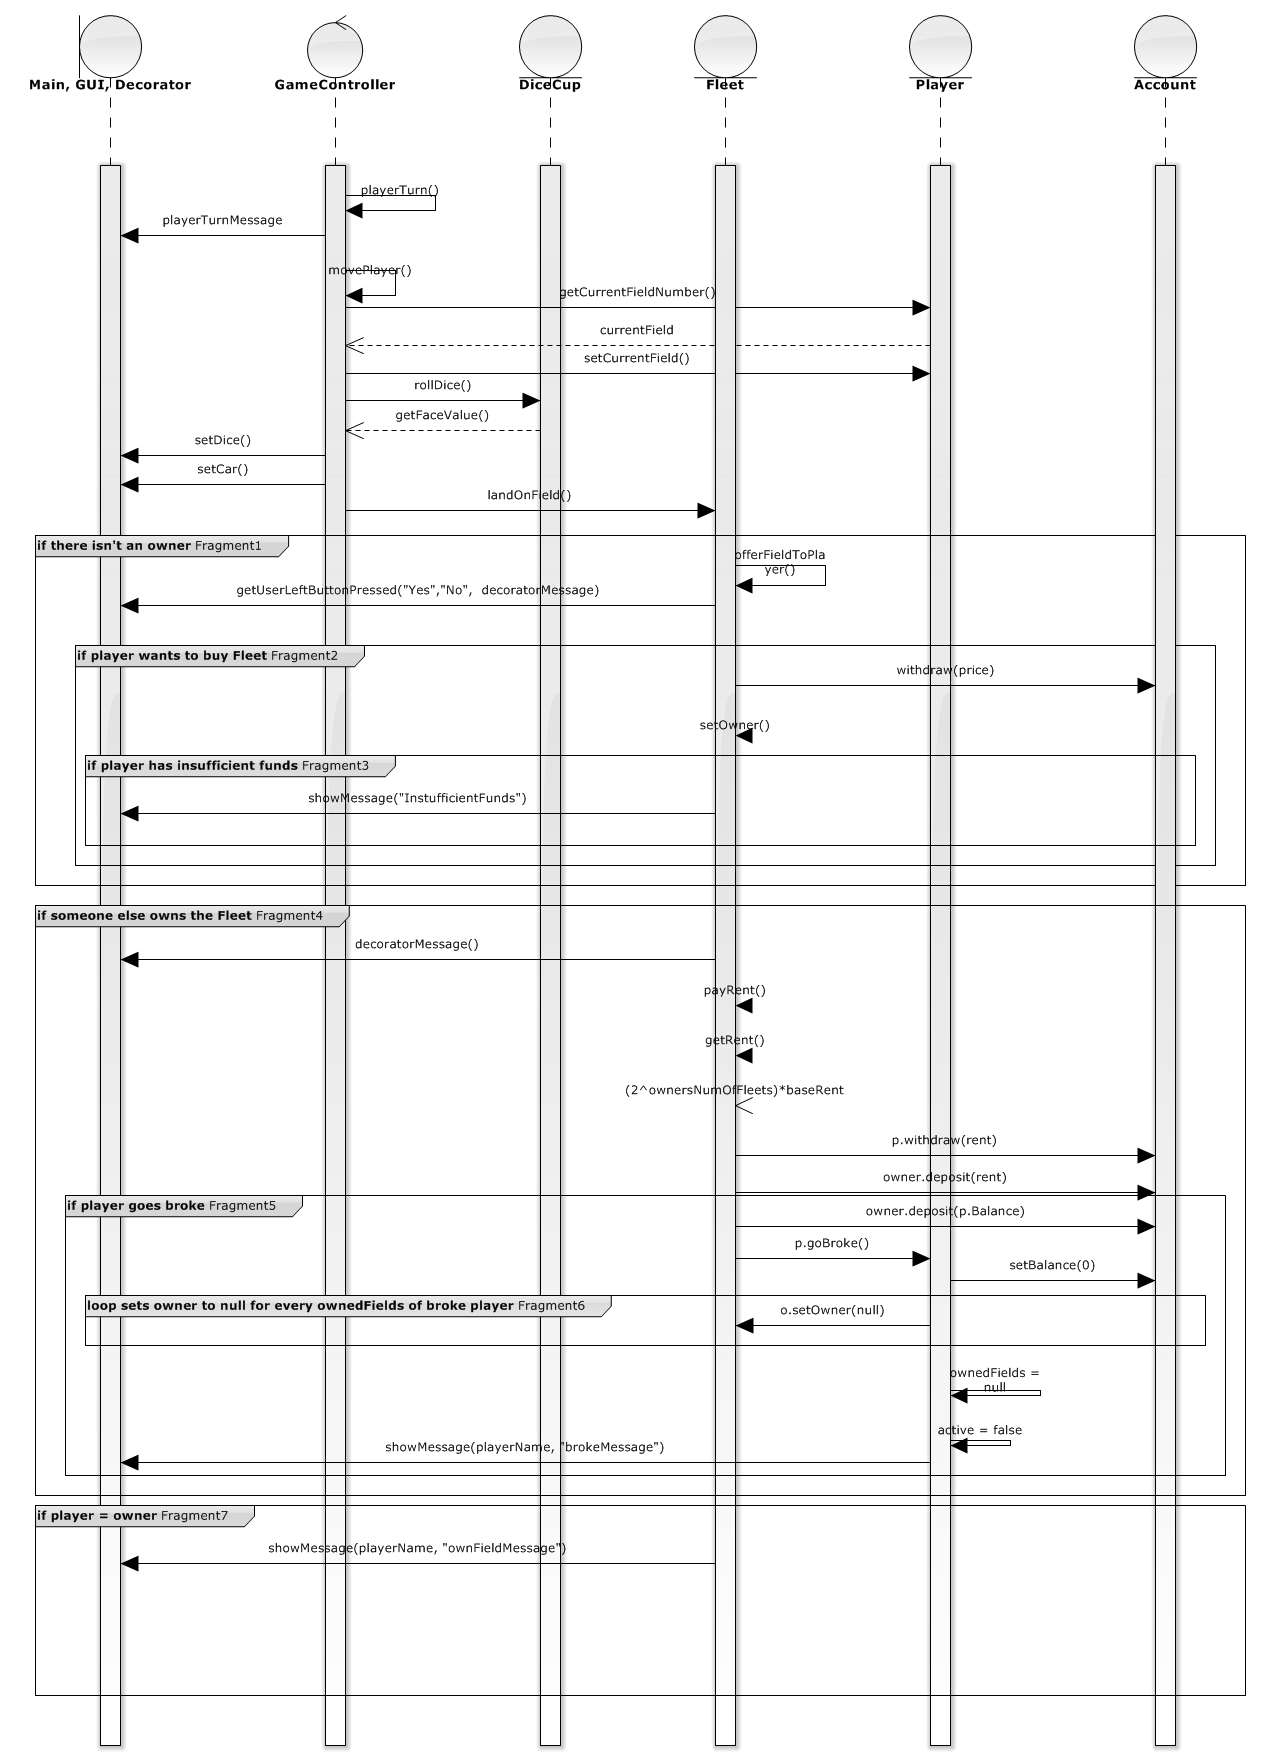
\includegraphics[width=\linewidth]{Sequencediagram3}
\caption{\emph{Sekvensdiagram 2}: Land on Field.}
\end{figure}
\FloatBarrier
Sekvensdiagrammerne er blevet lidt forsimplet for at fremme forståelse, og for
at ikke få for mange metodekald, der ikke ville bidrage til forståelsen af
diagrammet. Klasser der fungerer sammen og/eller ensartet er slået sammen.
Klasser af begrænset vigtighed for diagrammerne er også udeladt. Shuffler
indeholder en statisk metode, der blander felterne i starten af spillet. DiceCup
og Die arbejder så tæt sammen, at Die er undladt. Die er, som navnet hentyder,
en terning. Ownable er en superklasse til alle typer af felter, der kan ejes.
Fields er en superklasse til alle typer af felter. De forskellige typer af
felter, er slået sammen i det første diagram, og er kaldt Ownables, og i det
andet diagram, hvor vi viser landOnFleet, har vi valgt at udelukke de andre
felter, og ladt Fleet være den Ownable vi modellerer, da den er en subklasse af
“Ownable”. Mange returns er også blevet undladt for overskueligheden. Der er
brugt tre forskellige ikoner for klasser, nemlig Boundary, Control og Entity
(BCE), og man kan skelne dem ad ved at Boundary ser ud som, at den rører ved en
væg, Control har en lille pil på sig, og Entity ser ud som den rører ved noget
gulv. Derudover er der brugt to typer kasser. Loops, som repræsenterer loops,
hvis køringspremisser eller formål er beskrevet i den lille tekstboks øverst i
firkanten. Det andet er alt, som er kort for alternate. Dette viser et andet
udfald, der kan ske. Det bliver brugt til at vise ‘if’s og øverst i boksen er
præmissen for det givne if-alternativ anført.\\
\indent Det første sekvensdiagram viser et overordnet forløb af programmet, mens
det andet diagram viser alle de forskellige udfald, der kan opstå, når en spiller
lander på et  felt af typen Fleet. I det første er det på et lidt højere niveau
end i det  andet, da vi i det andet graver helt ind og ser på alle de
forskellige ting, der  kan ske, og ender derved med seks alternate-bokse.\\
\indent Hvis en spiller lander på en Fleet, er der allerede tre muligheder. Hvis
ingen ejer Fleet, skal det tilbydes til spilleren, hvorefter han kan vælge om han vil
købe den eller ej,  men der er en ekstra mulighed i det, at han måske ikke har
penge nok.\\
\indent Mulighed nummer to er, at en anden spiller ejer den. Så skal rent regnes
sammen, flyttes, og vi må se om spilleren er gået fallit. Hvis han er det, skal 
spilleren smides ud af spillet, og hans felter skal frigøres.\\
\indent Mulighed nummer tre er, at han selv ejer feltet, og så skal han bare
have en besked om, at han er landet på sit eget felt.
\section*{GRASP patterns}
\addcontentsline{toc}{subsection}{GRASP patterns}
Vi har forsøgt at arbejde med ‘responsibility driven design’ og implementeret
Controller, Creator, Information Expert, Low Coupling, High Cohesion og
Polymorphism.\\
\indent \emph{Controller} paradigmet er søgt overholdt ved vores GameController
klasse, der håndterer al spil logik og delegerer ansvaret videre. I vores projekt har vi
en lidt speciel statisk GUI, der tillader at vi tilgår den fra alle klasser i
programmet. Da den algoritme som felterne bruger er afhængig af spillerens
input fra GUI’en, har vi skullet vælge mellem at implementere 1) en løsning
hvor GameControlleren først tilgår feltet for at høre om det kan ejes, dernæst
om den kan købes eller er ejet, og dernæst eventuelt sætter ejeren for feltet,
eller 2) som vi i stedet har valgt - en løsning hvor felterne optræder som
subcontrollere og selv tilgår GUI’en for at håndtere hvad netop det felt gør.
På den måde bryder vi bevidst med BCE paradigmet (I det felterne også er
entities), men opnår en mere overskuelig løsning kodemæssigt og da relationen
er en ‘use’ relation med GUI’en øger det ikke coupling væsentligt. Cohesion
bevares også, da det er felterne selv, der logisk set kender reglerne for hvad
der sker når en spiller lander på feltet. Det er muligt at genskabe BCE, ved at
hvert felt får sin egen controller (hvilket ville være Pure Fabrication), men i
det givne tilfælde er det meget begrænset hvad en entity klasse skulle
indeholde, hvorfor vi har valgt at undlade at splitte klasserne op.\\
\indent \emph{Creator} er søgt overholdt ved at de klasser der ‘contains’ eller
‘aggregates’ andre klasser, også har ansvar for at instantiere dem. GameControlleren
instantierer DiceCup, der igen instantierer Die. Ligeledes oprettes Player med
account og Board med Fields. Vores Boundary klasse er et specialtilfælde, da den
er statisk, men initialiseres af GameControlleren, der har hovedansvaret for at
interagere med den.\\
\indent \emph{Information Expert} er søgt overholdt, ved kun at bevare
information og referencer i én klasse - den der er den mest oplagt til at indeholde
informationen. Vi har brudt med paradigmet enkelte steder for at opnå en mere
overskuelig løsning. Således har Gamecontrolleren en integer (playersLeft), der
holder styr på hvor mange players der er tilbage. Denne information er dubleret
fra players, der selv holder styr på om de er med i spillet med deres boolean
active. På samme måde ved både felterne hvem der ejer dem og playerne ved hvilke
felter de ejer. Dette giver desuden en højere coupling - da der er en reference
begge veje - Det giver også en lavere cohesion, da det nu er spredt over to
klasser. Man kan argumentere for at det stadig er logisk, da en grundejer kender
sine grunde og skødet på grunden ligeledes er påtrykt en ejer. Vi gør det under
alle omstændigheder for at opnå en simplere implementering af Fleet, der er nødt
til at vide hvor mange fleets ejeren har. Alternativet er at Fleet skal modtage
en reference til board og iterere over alle felterne for at afgøre hvor mange
fleets ejeren har. Et andet alternativ er at oprette en skødedatabase som kan
adspørges når behovet opstår - det ville svare til GRASP konceptet indirection
(og pure fabrication).\\
\indent \emph{Low Coupling} er opnået ved få koblinger pr. klasse - Dice er
koblet til DiceCup, Account til Player og Fields til Board, der igen er koblet
til GameController (se klasse diagram). GameControlleren har naturligt lidt
højere coupling - da  Dicecup, Players og Board (og Decorator) alle har
betydning for game-flowet. Det  er et acceptabelt antal bindinger - der
understøtter high cohesion. Vi  implementerer en undtagelse med et specifikt
felt - ‘Labor Camp’, der har en  reference til DiceCup. Det er gjort for at
kunne beregne lejen - uden at skulle  passe summen af øjne til feltet. En
alternativ løsning kunne være at  implementere DiceCup som en Singleton, der
kunne tilgås globalt. Som allerede  nævnt har vi en ‘use’ relation fra alle
felttyperne til GUI - idet de tilgår GUI  for at spørge spilleren om han vil
købe grunden eller betale et fast beløb eller  procent af formue i skat. Da det
er en ‘use’ relation er coupling stadig lav.\\
\indent \emph{High cohesion} er forsøgt bevaret ved at klassernes ansvarsområder
er nært beslægtede. Således har Die kun ansvar for terningernes øjne og at ‘slå’ et nyt
tilfældigt slag. Dicecup håndterer summen af øjnene og relaterede opgaver og så
fremdeles. Dette er i høj grad understøttet af low coupling, hvilket også
afspejles i at vi bryder med high cohesion samtidig med at vi bryder med low
coupling i tilfældet med ejerskabet af fields (som beskrevet ovenfor under
information expert)\\
\indent \emph{Polymorphism} er implementeret i vores felter. Her er
ensartede klassers kode forsøgt samlet i superklasser, således at vi genbruger
kode i højest muligt omfang og undgår at skrive den samme kode to gange. Det
afspejles tydeligst i decoratorMessage() metoden, der nedarver i 2 niveau og
sammensætter en ensartet besked til spilleren, sammensat af en besked om hvilket
felt man er landet på (bestemt af Field), en besked der afhænger af om feltet
kan ejes (bestemt af Ownable) og en besked fra selve feltet. Dette understøtter
reusability, idet ændringer i koden kun skal indføres et sted.

\chapter{Implementering}
\section{Klasser}
\subsection{Main}
\subsection{Player}
\subsection{Account}
\subsection{Decorator}
\subsection{DiceCup}
\subsection{Die}
\subsection{GameController}
\subsection{Board}
\subsection{Field}
\subsection{Ownable}
\subsection{Tax}

\chapter{Test}
\section*{BrugerTest}
\addcontentsline{toc}{subsection}{BrugerTest}
Vi har kørt nogle bruger tests, for at se om spillet opfører sig som forventet.
Vi har forsøgt at finde de fejl som gør at spillet af en eller anden grund giver
et forkert output, så som at spiller ikke går fallit når han skal, men får lov
at spille videre. Under \textbf{Bilag} kan man se screenshots fra en
brugertest.\\
\indent Under gennemførelsen af en brugertest, så det ud som at en vinder ikke
ikke blev præsenteret for spillerne. For at checke om controlleren kørte loopet
som finder vinderen, addede vi nogle linjer som blev printet hvis dele af loopen
blev kørt. Da vi så kørte den sidste brugertest fandt vi ud af at vinderen altid
spiller 1 selv om denne spiller var gået fallit
\textbf{\hyperref[bilag9]{Bilag9}}.
Fejlen var at da vi havde tilføjet den linje som blev printet, så havde vi glemt at omslutte if
statement med “\{“ således at alle spillere for den sags skyld kunne være
vindere. Ellers har vi kørt en fuldkommen brugertest hvor vi kommer igennem alle
scenarier vi kunne komme i tanker om. Bilag 1-9 er de scenarier vi forventer når
vi lander på et felt. Hvis man lander på et felt som ikke har en ejer, kan man
vælge at købe det, eller lade være \textbf{\hyperref[bilag1]{Bilag1}}.\\
\indent Hvis en spiller lander på et felt som er ejet af en anden, så får man
ikke mulighed for at købe det, men skal betale til ejeren
\textbf{\hyperref[bilag2]{Bilag2}}. Man kan også se at navnet på feltet og
navnet som bliver præsenteret som ejer af feltet er det samme. Det er den gule bil
(Christian) som er endt på Magnus felt og skal betale ham leje.\\
\indent Når man lander på det ene af tax felterne skal man have 2 muligheder for
at betale (enten 10\% eller 4000kr) \textbf{\hyperref[bilag7]{Bilag7}}. Mens det
andet tax felt kun skal kræve et bestemt beløb
\textbf{\hyperref[bilag3]{Bilag3}}. Disse felter får man ikke mulighed for at
købe, ligesom refugee heller ikke kan købes, men her får man penge
\textbf{\hyperref[bilag4]{Bilag4}}.\\
\indent Et andet scenarie er hvis du lander på dit eget felt, så skal der ikke
ske spilleren noget. Spilleren skal kun få at vide at han er landet på sit eget
felt \textbf{\hyperref[bilag5]{Bilag5}}, her kan nævnes at vi har gjort således
at felterne på GUI’en opdateres så man kan se hvem er ejer af feltet. Det er også
aktuelt når en spiller går fallit, så bliver den spiller fjernet som ejer af de
felter han havde og andre spillere får mulighed for at købe det
\textbf{\hyperref[bilag6]{Bilag6}}.\\
\indent Vi skulle også håndtere at en spiller ikke kan købe et felt for så at gå
fallit fordi han ikke har penge nok, og dette håndtere spillet
\textbf{\hyperref[bilag8]{Bilag8}}.
Spilleren får at vide at han ikke har penge nok, og spillet kører videre. dog
kan spilleren godt gå fallit når han lander på tax feltet hvor man vælge mellem
10\% og 4000 kr. Hvis han har råd til det ene, men ikke det andet, kan han
alligevel gå fallit ved forkert valg.\\
\indent To fejl som vi fandt ved brugertest, men som ikke er rettet, er hvis man 
skriver et grotesk langt navn for en spiller. Navnet bliver så langt at når det er
spillerens tur, dækker navnet “OK” knappen, og spillet kan ikke fortsættes
\textbf{\hyperref[bilag10]{Bilag10}}. Det skal altså være et virkelig, virkelig
langt navn. Hvis spillerne beslutter sig for at have samme navn, så bliver bliver to spillere
oprettet med hver sin konto, men på GUI’en har de samme farve bil
\textbf{\hyperref[bilag11]{Bilag11}}, altså er der kun en bil på brættet, men
som alligevel har to destinationer. Man kan derfor kun se bilen og balancen for den
ene spiller ad gangen.
\section*{Black Box (Junit)}
\addcontentsline{toc}{subsection}{Black Box (Junit)}
Vi har lavet en JUnit test class FieldJUnitTest, der tester LandOnField for alle
vores forskellige Field-klasser. Den opretter først sin egen test GUI, den skal
bruges da der er brugerinput i LandOnField, og derefter kører den en @test for
hver Field-type. Indlejret i disse test er også nogle test på ting fra Ownable,
såsom at gå fallit og lande på ens eget felt.\\
\indent Vi har kørt FieldJUnitTest løbene og brugt den til at rette adskillige
logiske fejl, til et punkt hvor FieldJUnitTest nu kører fejlfrit.
\section*{FURPS+}
\addcontentsline{toc}{subsection}{FURPS+}
FURPS+ er en forkortelse for Functionality, Usability, Reliability, Performance,
Supportability. FURPS+ er en god checkliste for at opnå et så godt program som
muligt, og ikke glemme nogle vigtige dele.
\begin{itemize}
  \item \textbf{functionality:} Vi har lavet et funktionelt spil, som opfylder
  alle kode mæssige krav, som for eksempel at bruge arv når vi programmerede felt
  klasserne og metoden landOnField i klassen Field.
  \item \textbf{Usability:} Spillet er brugervenligt, og der behøves ikke at
  læses nogen brugervejledning for at kunne gennemføre spillet. Dog skal man
  kende noget til matador regler for at forstå spillet, men du gennem spillet
  skal du kun trykke “OK” eller får du to valgmuligheder, hvor der er beskrevet
  hvad de betyder.
  \item \textbf{Reliability:} Gennem bruger tests og en stor J-Unit test, har vi
  elimineret alle de fejl, som opstår gennem de forventede scenarier. Som et af
  kravene har vi med J-Unit testet feltet af typen fleet for:
  \begin{itemize}
    \item at spiller ikke får fratrukket beløb når han lander på felt som han
    selv ejer.
    \item Når en spiller skal betale til en anden spiller, at den rigtige
    spiller får bestemt beløb og den anden fratrukket samme beløb.
    \item Når en spiller køber en fleet, bliver prisen af fleet fratrukket
    spillerens konto, og spiller bliver sat som ejer af feltet.
    \item Hvis en spiller er ejer af to fleets, så får den spiller som lander på
    en af hans fleet, fratrukket et beløb som svarer til $250 \cdot 2^(antal af
    fleets)$. Og ejeren tilføjet samme beløb.
    \item I tilfælde af at en spiller ikke har nok kapital ved landing på en
    andens spillers fleet, så bliver spillerens $balance = 0$, og
    $active = false$ (spilleren bliver inaktiv og er ikke mere del af
    spillet). Derefter bliver de penge som spilleren havde, overført til ejeren
    af fleet.
  \end{itemize}
  Så vi har et pålideligt spil, som ikke lukker ned uforventet.
  \item \textbf{Performance:} Dette har ikke været relevant faktor i vores spil.
  Spillet bruger så få ressourcer at vi har ikke haft brug for kørtids-analyser
  og optimering, spillet optager heller ikke mærkbar disk-space.
  \item \textbf{Supportability:} Vi har gjort en hel del ud af at fremtidssikre
  koden, så vi kan genbruge så meget som muligt af koden senere. For eksempel
  har vi undgået “hard coding”, og al tekst i spillet bliver gennem identifiers
  oversat, ved hjælp af decorator og properties filer, til meningsfyldt tekst.
  Properties filerne indeholder al tekst, og det gør det nemt at have overblik
  og ændre på teksten. Vi stødte dog på et problem, som vi løste med gøre
  felterne til subcontrollere, det gør koden lidt sværere at vedligeholde, da
  små ændringer i Decorator kan gøre at vi må gennemgå gamecontroller samt alle
  subcontrollerne for fejl.
  \item \textbf{+ (Plusset):} Spillet kræver at computeren har og kan køre en
  opdateret version af java og at mus og tastatur er tilkoblet. Spillet har
  ingen lyd, så det er ikke en nødvendighed. Ellers er der ikke nogen
  nævneværdige krav som spillet har til computeren.
\end{itemize}

\chapter{Konklution}
Vi har alt i alt fremstillet et spil, der funktionelt set lever op til
specifikationerne - og tilføjer ekstra funktionalitet. Det kan spilles med
begrænsede forkundskaber, om end et kendskab til reglerne er nødvendigt for at
få det optimale udbytte. Det er pålideligt, men mangler et tjek for
brugernavnenes længde - så det er muligt at ødelægge brugeroplevelsen for sig
selv ved at indtaste grotesk lange brugernavne.\\
\indent Vi har taget nogle designbeslutninger, der skaber højere kobling og
bryder med BCE paradigmet. Det giver en overskuelig kode, men skaber det problem at det er
sværere at vedligeholde, idet ændringer i Decorator kan skabe behov for
ændringer i flere forskellige klasser.\\
\indent Idet formålet var at undgå for meget kode i vores GameController, kan
man forsøge at opnå det samme ved at indføre en dedikeret FieldController, der
delegeres ansvaret for sub use casen ‘Land on Field’. Vores dobbelte kobling
mellem Player og felterne, kan evt. løses ved at indføre et
‘tinglysningsregister’ - en (singleton) klasse, der kun har til opgave at holde
styr på ejerskabet af fields.





More plain text.\cite{pear}	%%citering

test\cite{wikipedia}
\bibliography{51_del3_bib}%% her indsættes referencerne
\begin{appendices}
\FloatBarrier
\begin{figure}[h]
\section*{Bilag 1}\label{bilag1}
\centering
\makebox[\textwidth]{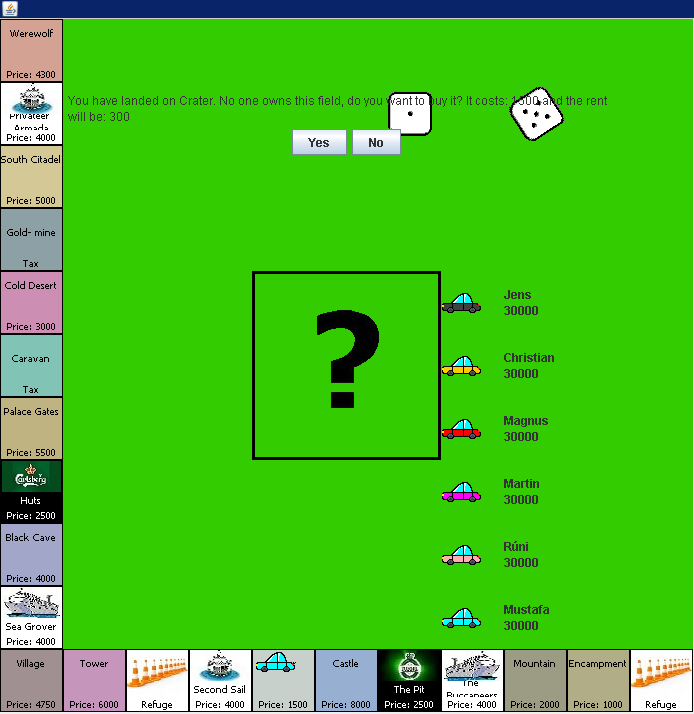
\includegraphics[width=0.8\paperwidth]{bilag01}}
\caption{\emph{Bilag 1}: Spilleren tilbydes at købe et felt.}
\end{figure}
\FloatBarrier
\begin{figure}[h]
\section*{Bilag 2}\label{bilag2}
\centering
\makebox[\textwidth]{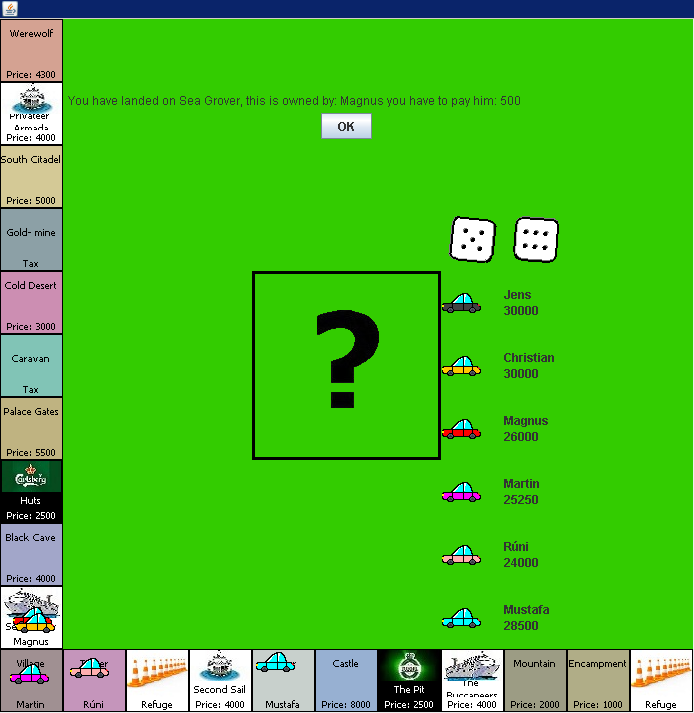
\includegraphics[width=0.8\paperwidth]{bilag02}}
\caption{\emph{Bilag 2}: Spilleren betaler leje.}
\end{figure}
\FloatBarrier
\begin{figure}[h]
\section*{Bilag 3}\label{bilag3}
\centering
\makebox[\textwidth]{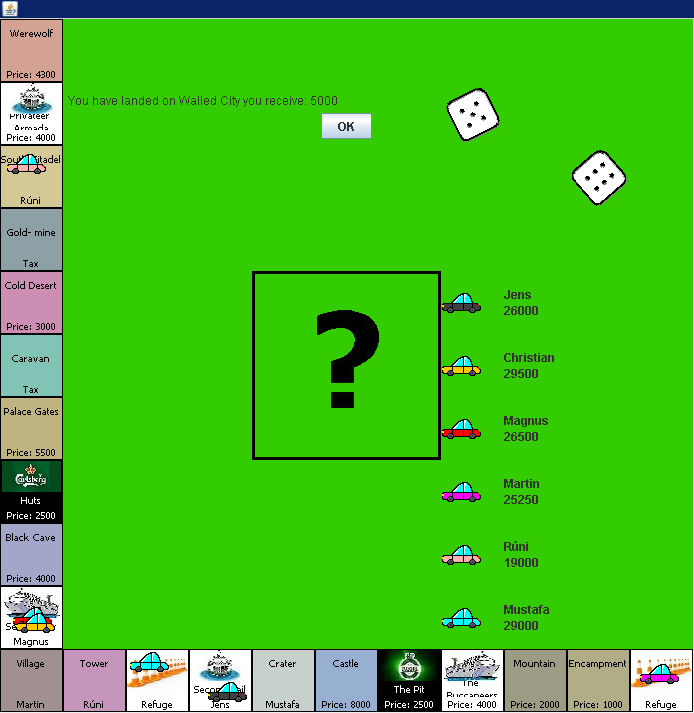
\includegraphics[width=0.8\paperwidth]{bilag03}}
\caption{\emph{Bilag 3}: Spilleren modtager penge på ‘Refuge’.}
\end{figure}
\FloatBarrier
\begin{figure}[h]
\section*{Bilag 4}\label{bilag4}
\centering
\makebox[\textwidth]{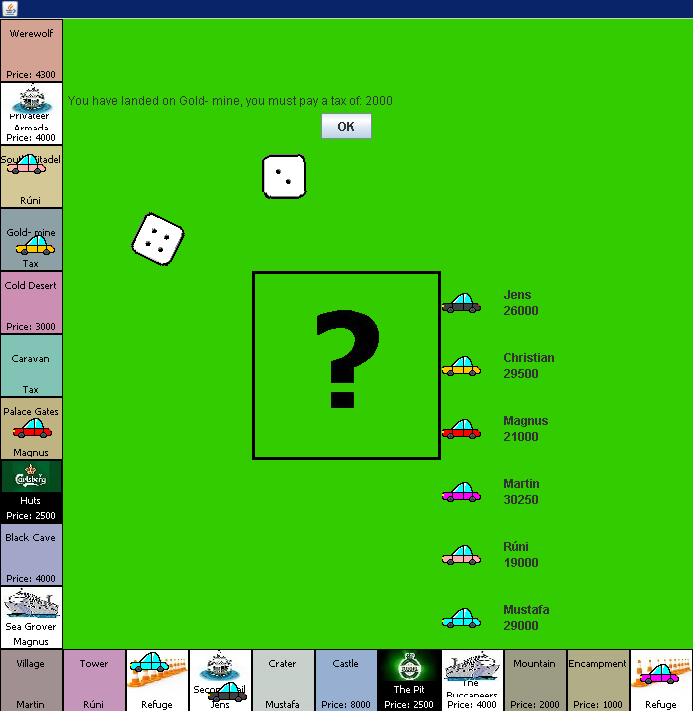
\includegraphics[width=0.8\paperwidth]{bilag04}}
\caption{\emph{Bilag 4}: Spilleren betaler fast skat på ‘Tax’.}
\end{figure}
\FloatBarrier
\begin{figure}[h]
\section*{Bilag 5}\label{bilag5}
\centering
\makebox[\textwidth]{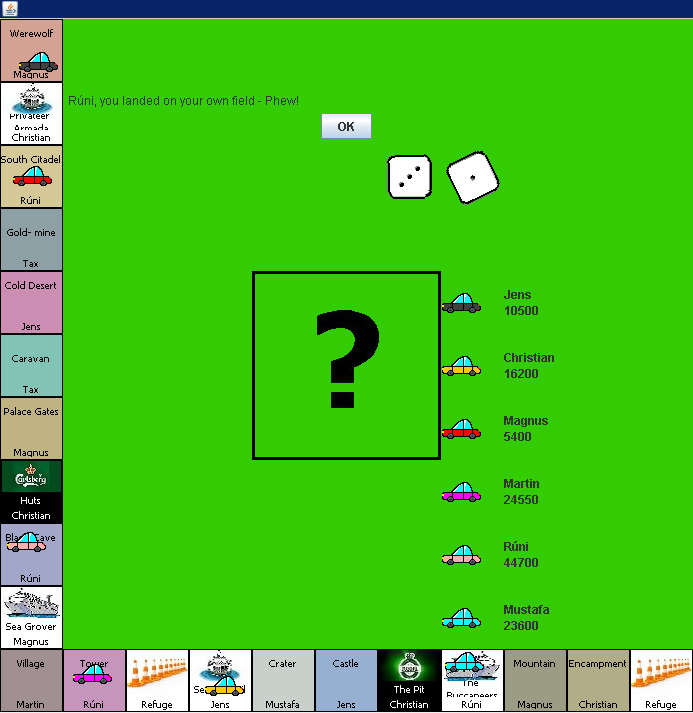
\includegraphics[width=0.8\paperwidth]{bilag05}}
\caption{\emph{Bilag 5}: Spilleren lander på eget felt.}
\end{figure}
\FloatBarrier
\begin{figure}[h]
\section*{Bilag 6}\label{bilag6}
\centering
\makebox[\textwidth]{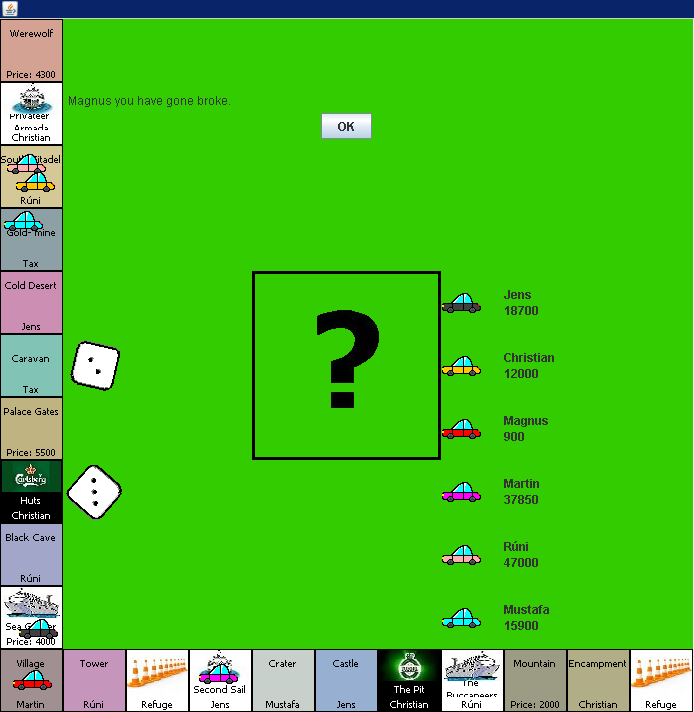
\includegraphics[width=0.8\paperwidth]{bilag06}}
\caption{\emph{Bilag 6}: Spilleren går fallit.}
\end{figure}
\FloatBarrier
\begin{figure}[h]
\section*{Bilag 7}\label{bilag7}
\centering
\makebox[\textwidth]{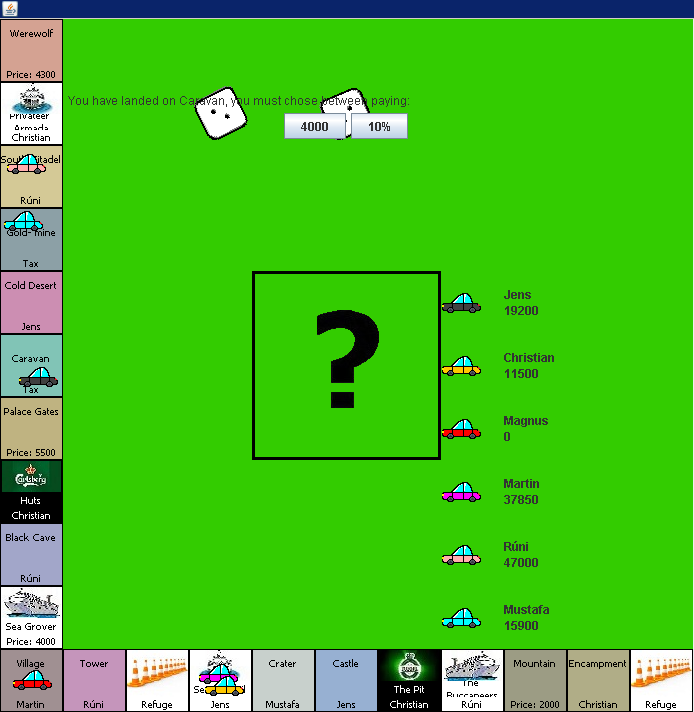
\includegraphics[width=0.8\paperwidth]{bilag07}}
\caption{\emph{Bilag 7}: Spilleren lander på et variabelt ‘Tax’ felt.}
\end{figure}
\FloatBarrier
\begin{figure}[h]
\section*{Bilag 8}\label{bilag8}
\centering
\makebox[\textwidth]{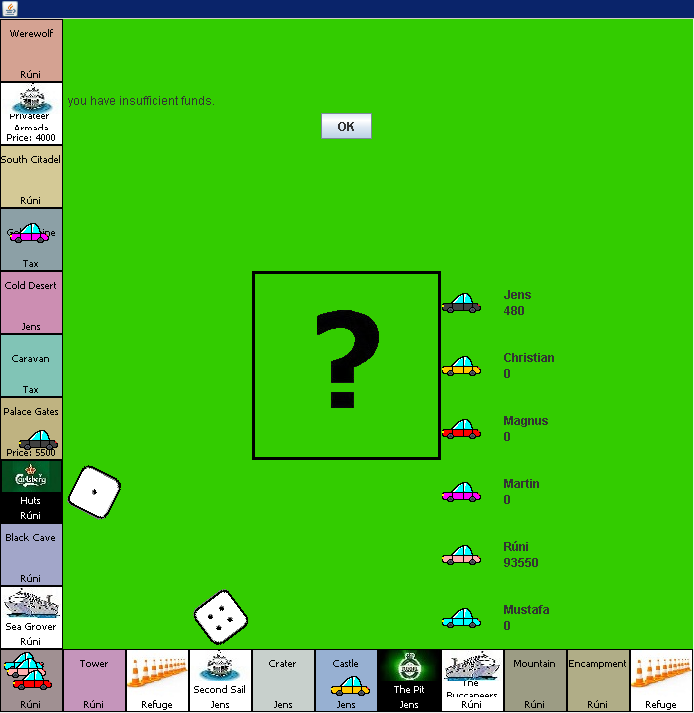
\includegraphics[width=0.8\paperwidth]{bilag08}}
\caption{\emph{Bilag 8}: Spilleren har ikke råd til at købe feltet.}
\end{figure}
\FloatBarrier
\begin{figure}[h]
\section*{Bilag 9}\label{bilag9}
\centering
\makebox[\textwidth]{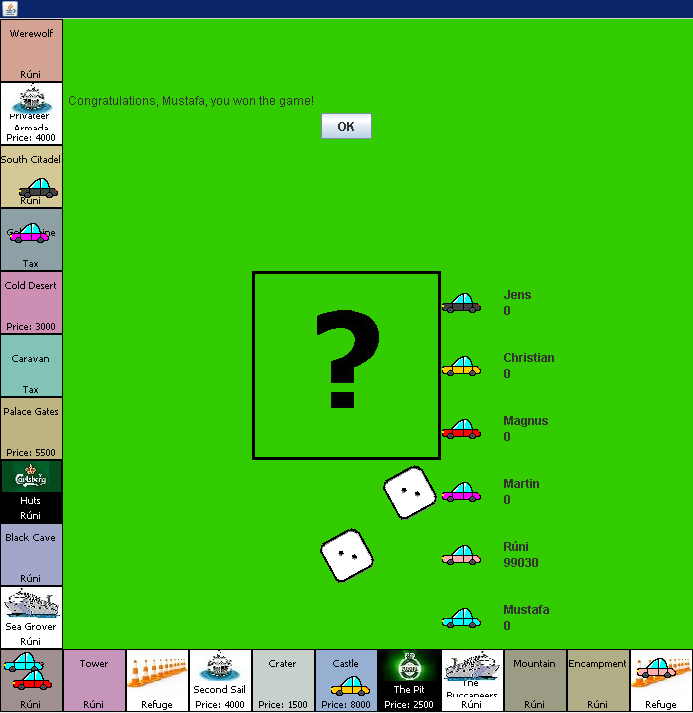
\includegraphics[width=0.8\paperwidth]{bilag09}}
\caption{\emph{Bilag 9}: Fejlagtig udnævnelse af vinderen - rettet i senere udgave.}
\end{figure}
\FloatBarrier
\begin{figure}[h]
\section*{Bilag 10}\label{bilag10}
\centering
\makebox[\textwidth]{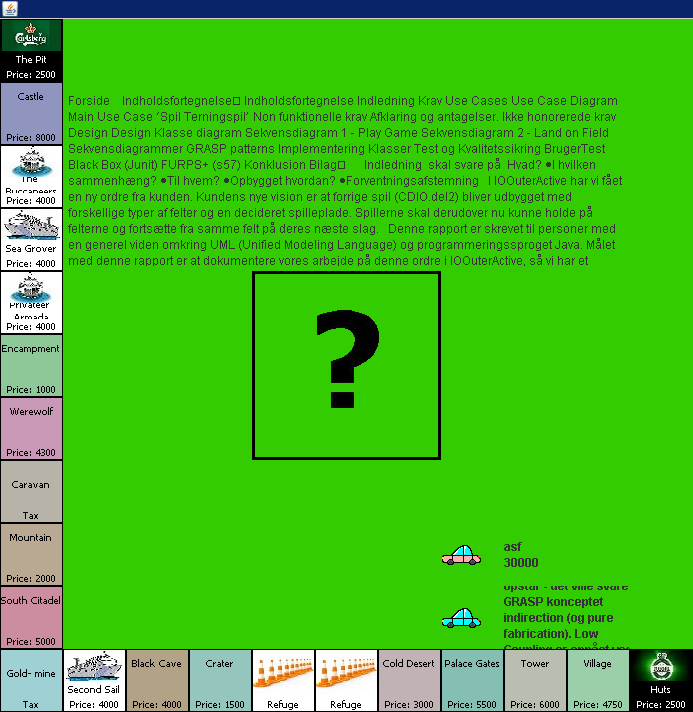
\includegraphics[width=0.8\paperwidth]{bilag10}}
\caption{\emph{Bilag 10}: Spilleren har valgt et meget langt navn - Hvilket får
ok knappen til at ‘forsvinde’ og gør spillet uspilleligt.}
\end{figure}
\FloatBarrier
\begin{figure}[h]
\section*{Bilag 11}\label{bilag11}
\centering
\makebox[\textwidth]{\includegraphics[width=0.8\paperwidth]{bilag11}}
\caption{\emph{Bilag 11}: Spillerne har valgt ens navne - Hvilket GUI’en ikke
kan håndtere.}
\end{figure}
\FloatBarrier
\end{appendices}
\end{document}
